\subsubsection{UC38 - Download dizionario dati}\label{UC38}

\begin{figure}[H]
  \centering
  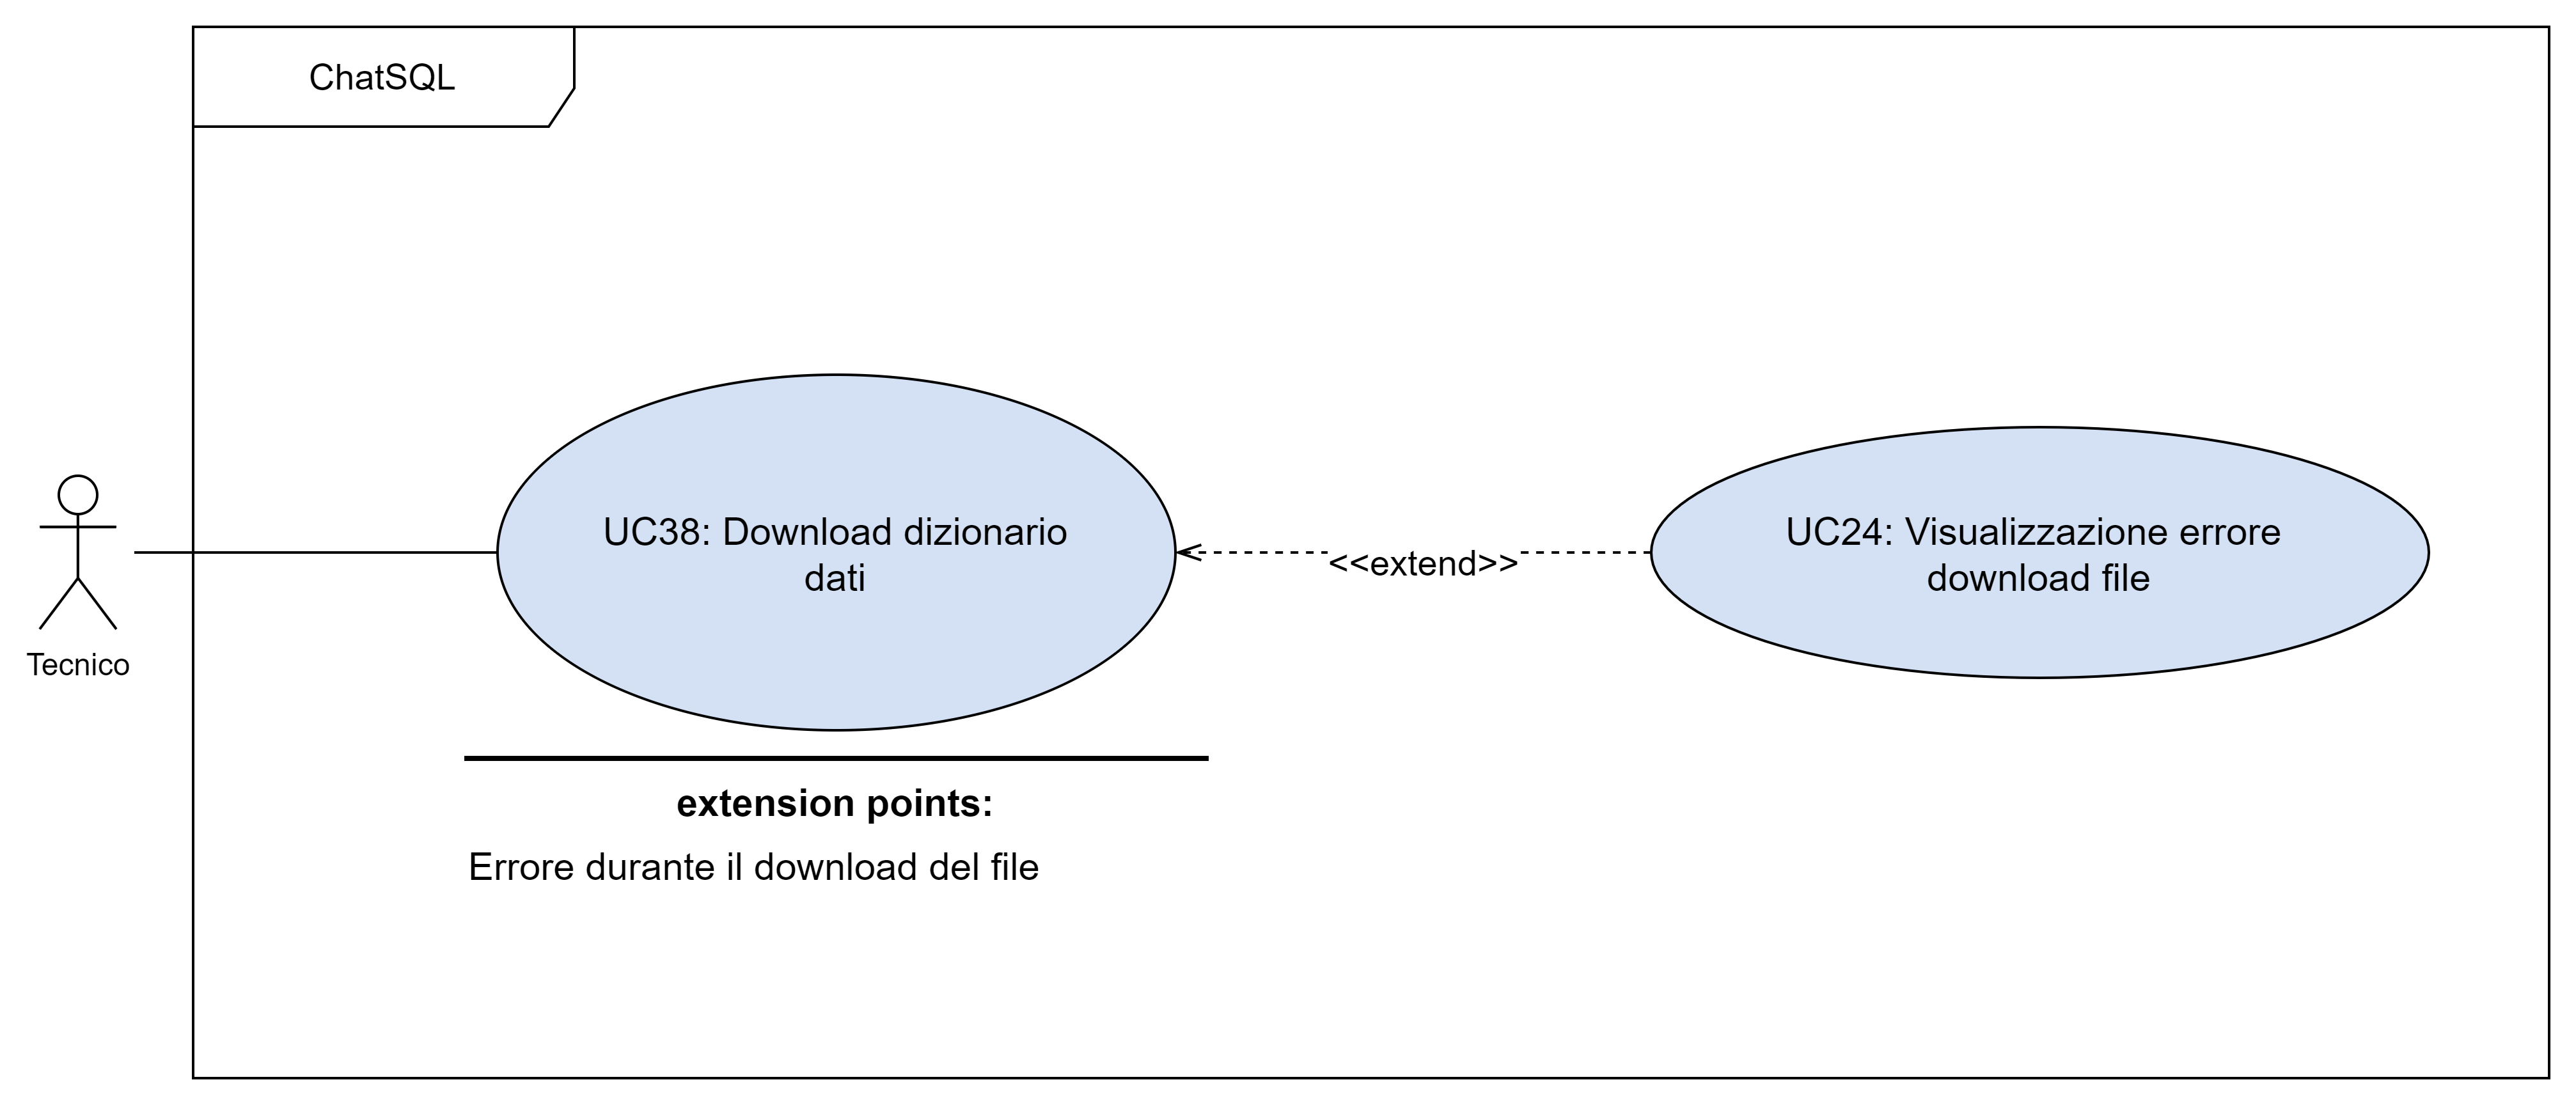
\includegraphics[width=0.95\textwidth]{assets/uc38.png}
  \caption{UC38}
\end{figure}

\paragraph*{Descrizione}
Il sistema consente al Tecnico di scaricare il file relativo a un \glossario{dizionario dati}.

\paragraph*{Attori principali}
Tecnico

\paragraph*{Precondizioni}
\begin{itemize}
  \item Il sistema è attivo e funzionante;
  \item Il Tecnico ha effettuato l'autenticazione (\hyperref[UC1]{UC1});
  \item Il Tecnico ha visualizzato la lista dei \glossario{dizionari dati} (\hyperref[UC9]{UC9});
  \item Il Tecnico ha individuato il dizionario da scaricare (\hyperref[UC9.1]{UC9.1}).
\end{itemize}

\paragraph*{Postcondizioni}
\begin{itemize}
  \item Il file è stato scaricato correttamente.
\end{itemize}

\paragraph*{Trigger}
Il Tecnico vuole scaricare un \glossario{dizionario dati}.

\paragraph*{Scenario principale}
\begin{enumerate}
  \item Il Tecnico richiede il download di un \glossario{dizionario dati};
  \item Il sistema esegue il download del file.
\end{enumerate}

\paragraph*{Scenario alternativo}
\begin{enumerate}
  \item Il sistema riscontra un errore durante il download del file (\hyperref[UC24]{UC24});
  \item Viene visualizzato un messaggio con i dettagli dell'errore.
\end{enumerate}

\paragraph*{Estensioni}
\begin{itemize}
  \item Visualizzazione errore download file (\hyperref[UC24]{UC24}):
  \begin{itemize}
    \item Extension point: Errore durante il download del file.
  \end{itemize}
\end{itemize}